\documentclass{beamer}

% === AUTOR === (((
\author{\textit{Por Erick I. Rodríguez Juárez.}}
% )))

% === PAQUETES === (((
% \usepackage{makeidx}
% \usepackage{xltxtra}
\usepackage{amsfonts}
\usepackage{amsmath}
\usepackage{amssymb}
% \usepackage{fullpage}
\usepackage{tikz}
\usetikzlibrary{arrows.meta}
\usepackage{graphicx}
% )))

% === TIPOGRAFÍA === (((
% \setmainfont[
  % BoldFont       = bodonibi,
	% ItalicFont     = Century modern italic2.ttf,
	% BoldItalicFont = bodonibi,
	% SmallCapsFont  = lmromancaps10-regular.otf
% ]{Century_modern.ttf}
% )))

% === COMANDOS === (((
% \newcommand{\dis}{\displaystyle}
% \newcommand{\qed}{\hspace{0.5cm}\rule{0.16cm}{0.4cm}}
% \newcommand{\operator}[1]{\mathop{\vphantom{\sum}\mathchoice
% {\vcenter{\hbox{\huge $#1$}}}
% {\vcenter{\hbox{\Large $#1$}}}{#1}{#1}}\displaylimits}
% \newcommand{\suma}{\operator{
\includegraphics[scale=0.09]{FOTOS/Sigma.png}}}
% \setlength{\parindent}{0mm}
% )))

% === ITALICA EN ENTORNO MATEMÁTICO === (((
% \DeclareSymbolFont{italics}{\encodingdefault}{\rmdefault}{m}{it}
% \DeclareSymbolFontAlphabet{\mathit}{italics}
% \ExplSyntaxOn
% \int_step_inline:nnnn { `A } { 1 } { `Z }
 % {  \exp_args:Nf \DeclareMathSymbol{\char_generate:nn{#1}{11}}{\mathalpha}{italics}{#1} }
% \int_step_inline:nnnn { `a } { 1 } { `z } {  \exp_args:Nf \DeclareMathSymbol{\char_generate:nn{#1}{11}}{\mathalpha}{italics}{#1}}
% \ExplSyntaxOff
% )))

\begin{document}

\frame{\titlepage}

\section{Ley de Enfriamiento de Newton.} % (((
\begin{frame}[t]
	\frametitle{Ley de Enfiramiento de Newton.}
	\vspace{-5mm}
	\begin{block}{}
	Esta ley nos dice que la tasa de cambio de la temperatura de un cuerpo es proporcional a la diferenci de temperatura del cuerpo y la del medo que lo rodea. Plantear la E.D. que describe esta ley.
	\begin{table}[ht]
		\centering
		\color{blue!80}
		\begin{tabular}{rl}
			\(T(t)\) : & Temperatura del cuerpo al tiempo \(t\). \\[2mm]
			\(T_m\) : & Temperatura del medio.
		\end{tabular}
	\end{table}
	\[
		\iff \color{green!50!black} \underbrace{\color{black} \dfrac{dT}{dt} = - \color{red} \underbrace{\color{black} k} _{(+)} \underbrace{\color{black} (T-T_m),} _{(+)}} _\text{\color{green!50!black} E.D.O. \(1^{er}\) Orden, Lineal Variables Separables, Autónoma.}  \color{black} k>0.
	\]
	Como la E.D. es autónoma, hagamos su análisis cualitativo.
		\[
			\dfrac{dT}{dt} = -k(T-T_m) = f(T).
		\]
	\end{block}

\end{frame}
\begin{frame}[t]
	\vspace{-5mm}
	\begin{block}{}
		\(f(T) = 0 \iff -k(T-T_m) =0 \iff T-T_m=0\), \color{red} \fbox{\color{black} \(T=T_m\)}.
		\color{black}
		\[
			f(T) = \color{red} \underbrace{\color{black}-k} _{m} \color{black} T+ \color{red} \underbrace{\color{black} kT_m} _{b}
		\]
		Grafiquemos a \(f(T)\). \vspace{-5mm}
		\begin{figure}[ht]
			\centering
			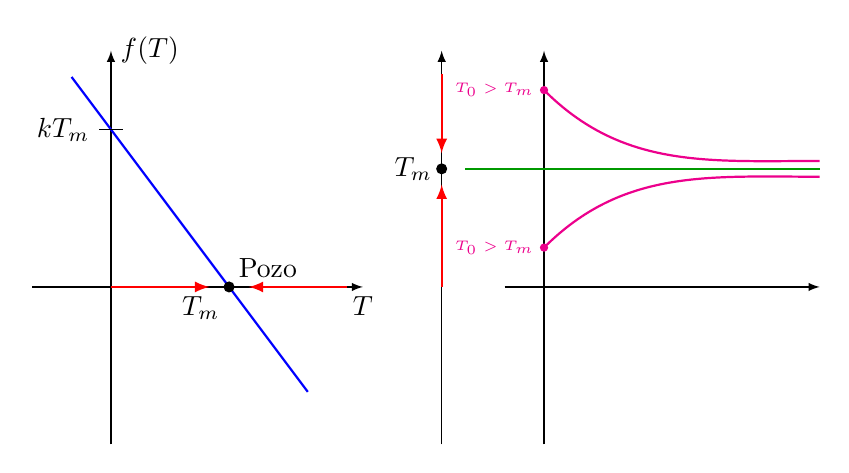
\begin{tikzpicture}[>=latex]
				\draw [->] (-1,0) -- (3.2,0) node [below] {\(T\)};
				\draw [->] (0,-2) -- (0,3) node [right] {\(f(T)\)};
				\draw [blue , thick , domain=-0.5:2.5] plot(\x , {2-1.333*\x});
				\fill (1.5,0) circle (2pt) node [above right] {Pozo} node [below left] {\(T_m\)};
				\draw [->, red, thick] (0,0) -- (1.25,0);
				\draw [->, red, thick] (3,0) -- (1.75,0);
				\draw (0.15,2) --++ (-0.3,0) node [left] {\(kT_m\)};
				\begin{scope}[xshift=4.5cm]
					\draw [->]  (0.5,0) -- (4.5,0);
					\draw [->] (1,-2) --++ (0,5);
					\begin{scope}[xshift=-3mm]
						\draw [->] (0,-2) --++ (0,5);
						\draw [thick, -> , red] (0,2.7) --++ (0,-1);
						\draw [thick, ->, red] (0,0) --++ (0,1.3);
						\fill (0,1.5) circle (2pt) node [left] {\(T_m\)};
					\end{scope}
					\draw [green!60!black, thick] (0,1.5) --++ (4.5,0);
					\draw [thick, magenta] (1,2.5) node [left] {\tiny \(T_0>T_m\)} to [out=-45 , in=180] (4.5,1.6); 
					\draw [thick, magenta] (1,0.5) node [left] {\tiny \(T_0>T_m\)} to [out=45 , in=-180] (4.5,1.4); 
					\fill [magenta] (1,0.5) circle (1.5pt);
					\fill [magenta] (1,2.5) circle (1.5pt);
				\end{scope}
			\end{tikzpicture}
		\end{figure}
	\end{block}
\end{frame}

\begin{frame}[t]
	\begin{block}{}
		Independintemente de la temperatura inicial del cuerpo, ésta tienda a la temperatura del medio.
	\end{block}
	\begin{example}
		Un termómetro que marca \(100^ \circ F\) se coloca en un medio con temperatura constante de \(70^ \circ F\). Después de \(6 min\) el temrómetro marca \(80^ \circ F\). ¿Cuál es la lectura después de \(20min\)? Además, determina en qué momento el termómetro marcará \(90^ \circ F\), \(75^ \circ F\), y \(69.9^ \circ F\).
	\end{example}
\end{frame}
\begin{frame}[t]
\end{frame}

\begin{frame}[t]
	\begin{figure}[ht]
		\centering
		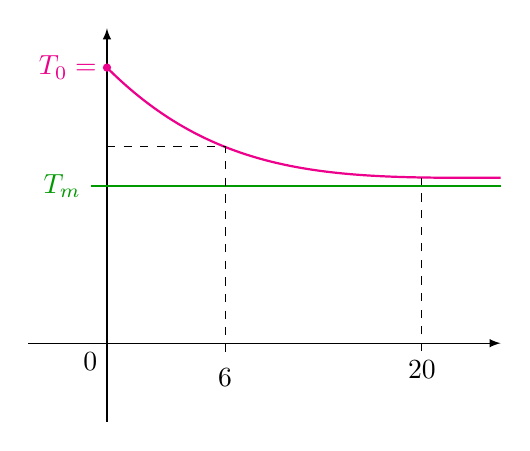
\begin{tikzpicture}[>=latex]
			\draw [->] (-1,0) -- (5,0);
			\draw [->] (0,-1) -- (0,4);
			\node [below left] at (0,0) {\(0\)};
			\draw [thick , green!60!black] (-0.2,2) node [left] {\(T_m\)} --++ (5.2,0);
			\draw [thick , magenta] (0,3.5) node [left] {\(T_0=\)} to [out=-45 , in=180] (5,2.1); 
			\fill [magenta] (0,3.5) circle (1.5pt);
			\draw [dashed] (0,2.5) --++ (1.5,0) --++ (0,-2.7) node [below] {\(6\)};
			\draw [dashed] (4,-0.1) node [below] {\(20\)} --++ (0,2.2);
		\end{tikzpicture}
	\end{figure}
\end{frame}

\begin{frame}[t]
	\begin{alertblock}{Ejercicio.}
		Era el medio día en un dá frío de Diciembre en Tampa, \(16^ \circ C\). EL detective Taylor llegó a la escena de crimen y halló al sargento revisando el cadáver. El sargento dijo que había varios sospechosos. Si supieran el momento exacto de la muerte podrían reducir la lista de sospechosos. EL detective Taylor sacó un termómetro y tomó la temperatura del cuerpo \(34.5^ \circ C\). Y luego salió a comer. Al regresar a la \(1:00pm\) halló que la temperatura del cuerpo era de \(33.7^ \circ C\). ¿En qué momento ocurrió el asesinato? (Considera la temperatura normal del cuerpo como \(37^ \circ C\)).
	\end{alertblock}
\end{frame}
\begin{frame}[t]
\end{frame}
% )))

\section{Caída Libre.} % (((
\begin{frame}[t]
\frametitle{Caída Libre.}
\begin{block}{}
	En experimentos con cuerpos de poca densidad, por ejemplo, una pluma, un copo de nieve, una pelota perforada, la resistencia del aire ejerce una furza sobre el cuerpo proporcional a su velocidad instantánea. Así pues, sobre ese cuerpo sólo actúan la resistencia del aire y la gravedad.\\[2mm]
	\begin{minipage}{0.4\linewidth}
		\centering
		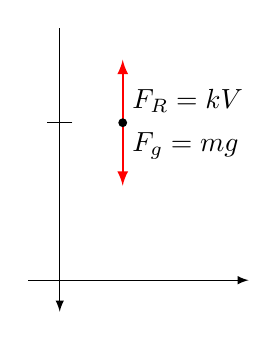
\begin{tikzpicture}[>=latex, scale=0.8]
			\draw [->] (0,4) -- (0,-0.5);
			\draw [->] (-0.5,0) -- (3,0);
			\draw (0.2,2.5) --++ (-0.4,0);
			\draw [red ,thick ,<->] (1,1.5) --++ (0,2);
			\fill (1,2.5) node [above right] {\(F_R = kV\)} node [below right] {\(F_g=mg\)} circle (2pt);
		\end{tikzpicture}
	\end{minipage}\hspace{5mm}
	\begin{minipage}{0.5\linewidth}
		La fuerza total que actúa sobre el objeto es:
		\[
			F_T = F_g - F_R = mg - kV.
		\]
		Por la \(2^{da}\) Ley de Newton
		\[
			F_T = ma = m \dfrac{dV}{dt}.
		\]
	\end{minipage}
\end{block}
\end{frame}

\begin{frame}[t]
	\begin{block}{}
		Igualando
		\[
			m \dfrac{dV}{dt} = mg-kV,
		\]
		\[
			\iff \hspace{5mm} \color{red} \fbox{\color{black} \(\dfrac{dV}{dt} = g- \dfrac{k}{m} V\)} \hspace{5mm} \color{black} k,m,g >0.
		\]
		\hspace{1.5cm} \color{red} E.D.O, \(1^{er}\) Orden, Lineal, V.S., Autónoma. \\
		\color{black} Como la E.D. es autónoma, hagamos su análisis cualitativo: \vspace{-5mm}
		\[
			\dfrac{dV}{dt} = g- \dfrac{k}{m} V = f(V).
		\]
		Obtengamos los puntos de equilibrio \vspace{-5mm}
		\[
			\begin{array}{rcl}
				f(V) =0 & \iff & g- \dfrac{k}{m} V =0 \\[2mm]
				& \iff & \dfrac{k}{m} V=g \\[2mm]
				& \iff & V = \dfrac{mg}{k}.
			\end{array}
		\]
	\end{block}
\end{frame}

\begin{frame}[t]
	\begin{block}{}
		\(\therefore\) \(V(t) = \dfrac{mg}{k}\) es solución de equilibrio.
		\begin{figure}[ht]
			\centering
			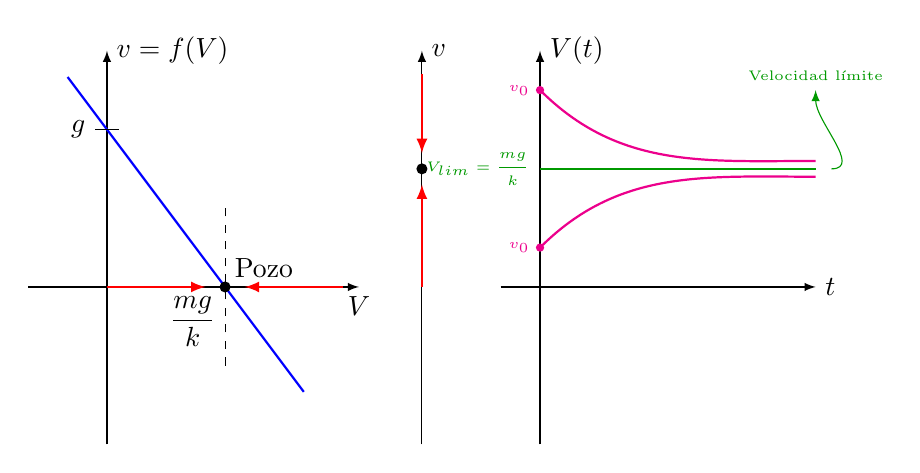
\begin{tikzpicture}[>=latex]
				\draw [->] (-1,0) -- (3.2,0) node [below] {\(V\)};
				\draw [->] (0,-2) -- (0,3) node [right] {\(v=f(V)\)};
				\draw [blue , thick , domain=-0.5:2.5] plot(\x , {2-1.333*\x});
				\fill (1.5,0) circle (2pt) node [above right] {Pozo} node [below left] {\(\dfrac{mg}{k}\)};
				\draw [dashed] (1.5,-1) --++ (0,2);
				\draw [->, red, thick] (0,0) -- (1.25,0);
				\draw [->, red, thick] (3,0) -- (1.75,0);
				\draw (0.15,2) --++ (-0.3,0) node [left] {\(g\)};
				\begin{scope}[xshift=4.5cm]
					\draw [->]  (0.5,0) -- (4.5,0) node [right] {\(t\)};
					\draw [->] (1,-2) --++ (0,5) node [right] {\(V(t)\)};
					\begin{scope}[xshift=-5mm]
						\draw [->] (0,-2) --++ (0,5) node [right] {\(v\)};
						\draw [thick, -> , red] (0,2.7) --++ (0,-1);
						\draw [thick, ->, red] (0,0) --++ (0,1.3);
						\fill (0,1.5) circle (2pt);
					\end{scope}
					\draw [green!60!black, thick] (1,1.5) node [left] {\tiny \(V_{lim} = \dfrac{mg}{k}\)} --++ (3.5,0);
					\draw [green!60!black,->] (4.7,1.5) to [out=0 , in=-90] (4.5,2.5) node [above] {\tiny Velocidad límite}; 
					\draw [thick, magenta] (1,2.5) node [left] {\tiny \(v_0\)} to [out=-45 , in=180] (4.5,1.6); 
					\draw [thick, magenta] (1,0.5) node [left] {\tiny \(v_0\)} to [out=45 , in=-180] (4.5,1.4); 
					\fill [magenta] (1,0.5) circle (1.5pt);
					\fill [magenta] (1,2.5) circle (1.5pt);
				\end{scope}
			\end{tikzpicture}
		\end{figure}
	\end{block}
\end{frame}

\begin{frame}[t]
	\begin{example}
		Un objeto de \(5\;kg\) es liberado desde el reposo a \(500\;m\) del suelo. Suponga que la fuerza de gravedad es de \(9.81\;m/s^2\), y es constante, y que la fuerza de resistencia del aire es proporcional a la velocidad del objeto con \(k=3\;kg/s\). Encuentre la función de velocidad y la función del movimiento. Además determine
		\begin{enumerate}
			\item ¿Cuál es la velocidad límite del cuerpo?
			\item ¿Cuándo alcanza la velocidad límite?
			\item ¿Qué velocidad lleva el objeo cuando choca contra el suelo?
		\end{enumerate}
	\end{example}
\end{frame}

\begin{frame}[t]
	\begin{enumerate}
		\item \(V_{lim} =\) ?
		\item \(t^* = \) ? tal que \(V(t^*) =V_{lim}\).
		\item \(t_1 )\) ? tal que \(x(t_1) =500\), \(V(t_1) =\) ?
	\end{enumerate}
	\begin{figure}[ht]
		\centering
		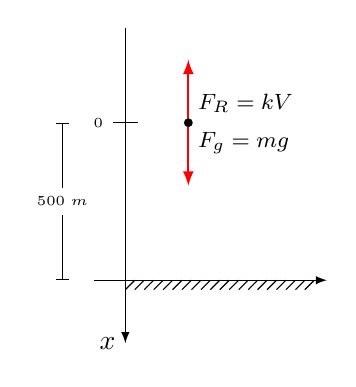
\begin{tikzpicture}[>=latex, scale=0.8]
			\draw [->] (0,4) -- (0,-1) node [left] {\(x\)};
			\draw [->] (-0.5,0) -- (3.2,0);
			\draw (0.2,2.5) --++ (-0.4,0) node [left] {\tiny \(0\)};
			\draw [|-|] (-1,2.5) to node[fill= white] {\tiny \(500\;m\)} (-1,0);
			\draw [red ,thick ,<->] (1,1.5) --++ (0,2);
			\fill (1,2.5) node [above right] {\footnotesize \(F_R = kV\)} node [below right] {\footnotesize \(F_g=mg\)} circle (2pt);
			\foreach \n in {1,...,20} \draw (3*\n/20,0) --++ (-0.15,-0.15);
		\end{tikzpicture}
	\end{figure}
\end{frame}
\begin{frame}[t]
\end{frame}

\begin{frame}[t]
	\begin{alertblock}{Ejercicio.}
		Un paracaidista y su paracaídas pesan \(92\;kg\). En el instante en el que el paracaídas se abre, él está viajando verticalmente a una velocidad de \(20\;m/s\). Si la fuerza debida a a resistencia del aire es proporcional a la velocidad instantánea con constante de proporcionalidad \(k=28\;kg/s\).
		\begin{enumerate}
			\item Encuentra la velocidad límite del paracaidista.
			\item Determina la posición y la velocidad para cualquier tiempo.
		\end{enumerate}
	\end{alertblock}
\end{frame}
\begin{frame}[t]
\end{frame}

\begin{frame}[t]
	Graficas:
	\begin{figure}[ht]
		\centering
		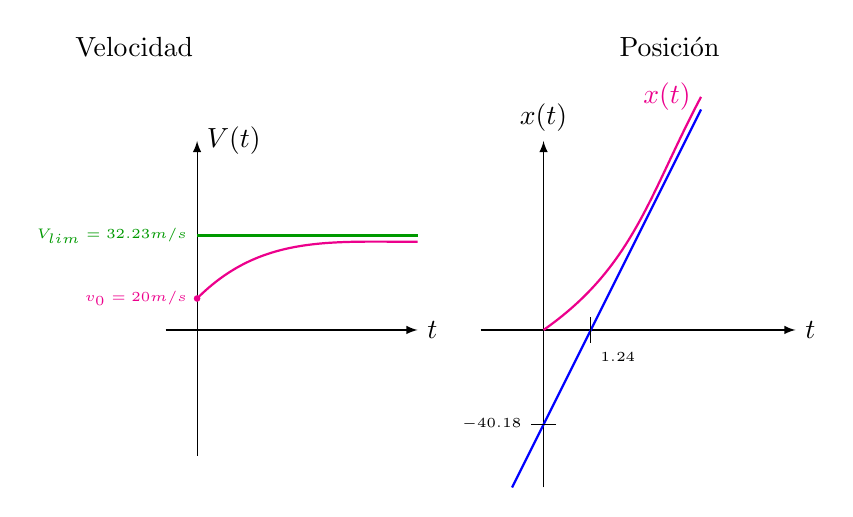
\begin{tikzpicture}[>=latex, scale=0.8]
			\draw [->]  (0.5,0) -- (4.5,0) node [right] {\(t\)};
			\draw [->] (1,-2) --++ (0,5) node [right] {\(V(t)\)};
			\draw [green!60!black, thick] (1,1.5) node [left] {\tiny \(V_{lim} = 32.23m/s\)} --++ (3.5,0);
			\draw [thick, magenta] (1,0.5) node [left] {\tiny \(v_0 = 20m/s\)} to [out=45 , in=-180] (4.5,1.4); 
			\fill [magenta] (1,0.5) circle (1.5pt);
			\node at (0,4.5) {Velocidad};
			\begin{scope}[xshift=6.5cm]
				\draw [->] (-1,0) -- (4,0) node [right] {\(t\)};
				\draw [->] (0,-2.5) -- (0,3) node [above] {\(x(t)\)};
				\draw [thick , blue, domain=-0.5:2.5] plot(\x , {2*\x-1.5});
				\draw [thick , magenta] (0,0) to [out=35, in =242] (2.5,3.7) node [left] {\(x(t)\)};
				\draw (0.75,0.2) --++ (0,-0.4) node [below right] {\tiny \(1.24\)};
				\draw (0.2,-1.5) --++ (-0.4,0) node [left] {\tiny \(-40.18\)};
				\node at (2,4.5) {Posición};
			\end{scope}
		\end{tikzpicture}
	\end{figure}
	\small \(V(t) = 32.23\underbrace{-12.23 e^{- \dfrac{7}{23} t}} _\text{termino transitorio}\), \hspace{3mm} \(x(t) = \underbrace{32.23-40.18} _\text{recta} + \underbrace{40.18 e^{- \dfrac{7}{23} t}} _\text{término transitorio}\).
\end{frame}
% )))

\section{Cable Colgante.} % (((

\begin{frame}[t]
	\frametitle{Cable Colgante.}
	\begin{block}{}
Considérese un cable flexible a ona cuerda que cuelga de los puntos \(A\) y \(B\), no-necesariamente al mismo nivel.
\begin{figure}[ht]
	\centering
	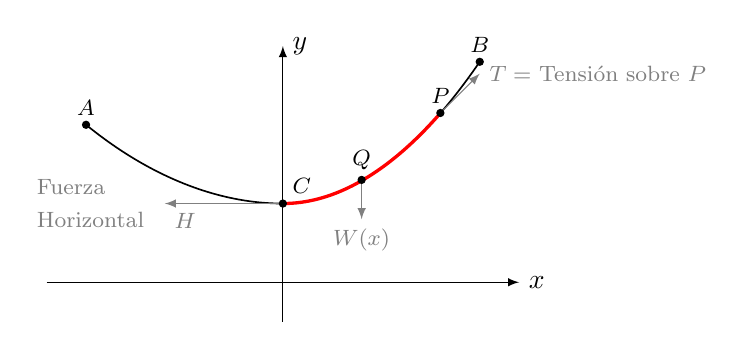
\begin{tikzpicture}[>=latex]
		\draw [->] (-3,0) -- (3,0) node [right] {\(x\)};
		\draw [->] (0,-0.5) -- (0,3) node [right] {\(y\)};
		\draw [semithick] (-2.5,2) parabola bend (0,1) (2.5,2.8);
		\begin{scope}
			\clip (0,0) rectangle (2,3);
			\draw [very thick , red] (-2.5,2) parabola bend (0,1) (2.5,2.8);
		\end{scope}
		\draw [->, gray] (0,1) --++ (-1.5,0) node [below right] {\footnotesize \(H\)} node [left, text width=1.5cm] {\footnotesize Fuerza Horizontal};
		\draw [->, gray] (1,1.3) --++ (0,-0.5) node [below] {\footnotesize \(W(x)\)};
		\draw [->, gray] (2,2.15) --++ (0.5,0.5) node [right] {\footnotesize \(T = \) Tensión sobre \(P\)};
		\fill (-2.5,2) circle (1.5pt) node [above] {\footnotesize\(A\)};
		\fill (2.5,2.8) circle (1.5pt) node [above] {\footnotesize\(B\)};
		\fill (0,1) circle (1.5pt) node [above right] {\footnotesize\(C\)};
		\fill (2,2.15) circle (1.5pt) node [above] {\footnotesize\(P\)};
		\fill (1,1.3) circle (1.5pt) node [above] {\footnotesize\(Q\)};
	\end{tikzpicture}
\end{figure}
Dado que la cuerda está en equilibrio, hagamos el balance de fuerzas.
\[
	\sum F_x =0 \hspace{1cm} \sum F_y =0.
\]
	\end{block}
\end{frame}

\begin{frame}[t]
	\begin{block}{}
	\begin{minipage}{0.5\linewidth}
		\begin{tikzpicture}[>=latex]
			\begin{scope}
				\clip (0,0) rectangle (2,3);
				\draw [very thick , red] (-2.5,2) parabola bend (0,1) (2.5,2.8);
			\end{scope}
			\draw [->, gray] (2,2.15) --++ (1,1) node [above left] {\footnotesize \(T\)};
			\draw [gray] (2,2.15) --++ (1,0) node [below left] {\tiny \(T \cos \theta\)} --++ (0,1) node [below right] {\tiny \(T \sin \theta\)};
			\draw [->, gray] (0,1) --++ (-1.5,0) node [below right] {\footnotesize \(H\)};
			\draw [->, gray] (1,1.3) --++ (0,-0.5) node [below] {\footnotesize \(W(x)\)};
			\draw [gray] (2,2.15)++(0.35,0)  arc (0:45: 0.35 cm) node [right] {\tiny \(\theta\)};
			\fill (0,1) circle (1.5pt) node [above right] {\footnotesize\(C\)};
			\fill (2,2.15) circle (1.5pt) node [above] {\footnotesize\(P\)};
			\fill (1,1.3) circle (1.5pt) node [above] {\footnotesize\(Q\)};
		\end{tikzpicture}\\[2mm]
		Por tanto
		\begin{flushright}
			\color{red} \fbox{\color{black} \(\dfrac{dy}{dx} = \dfrac{W(x)}{H}\)} \hspace{3mm}
		\end{flushright}
	\end{minipage}
	\begin{minipage}{0.4\linewidth}
		Luego:
		\[
			H = T \cos \theta \hspace{3mm} y \hspace{3mm} W(x) = T \sin \theta .
		\]
		Luego
		\[
			\dfrac{dy}{dx} = \tan \theta = \dfrac{T \sin \theta}{T \cos \theta } = \dfrac{W(x)}{H}. \vspace{8mm}
		\]
		\footnotesize
		E.D.O de Primer Orden.\\
		Lineal, V.S.\\
		\color{red} \underline{\color{black} \(y(0) =C\)}
	\end{minipage} \\[2mm]
		Derivemos la E.D. \vspace{-2mm}
		\[
			\color{red} \underline{\color{black} \dfrac{d^2y}{dx^2} = \dfrac{1}{H} \dfrac{dW}{dx}} \hspace{5mm}
			\color{black}
			\begin{array}{c}
				\mbox{E.D.O de } 2^{do} \mbox{ Orden} \\[2mm]
				\mu y(0) =C \;,\; y'(0) =0.
			\end{array}
		\]
	\end{block}
\end{frame}

\begin{frame}[t]
	\begin{block}{}
		\(\dfrac{dW}{dx} \;:\;\) representa el incremento en el peso por unidad de longitud en la dirección horizontal.
	\end{block}
	\begin{alertblock}{Ejercicio.}
		En los siguientes ejercicios veremos que para diferentes cargas por unidad de distancia horizontal obtenemos varias ecuacioones diferenciales las cuales producen varias formas del cable.
	\end{alertblock}
\end{frame}

\begin{frame}[t]
	\begin{example}
		Un cable flexible de poco a poco (despreciable) soporta un puente uniforme, ver la figura. Determine la forma del cable. Este es un problema de determinar la forma el cable en un puente colgante, el cuál, es de gran uso en la construcción moderna de puentes. \\[2mm]
	\end{example}
		\begin{minipage}{0.4\linewidth}
			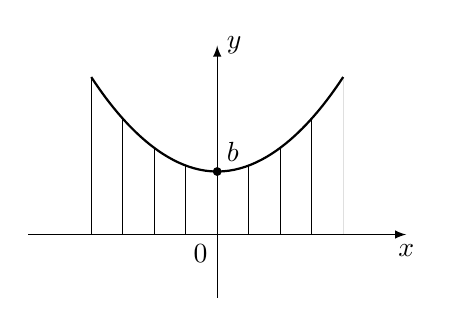
\begin{tikzpicture}[>=latex, scale=0.8]
				\draw [->] (-3,0) -- (3,0) node [below] {\(x\)};
				\draw [->] (0,-1) -- (0,3) node [right] {\(y\)};
				\draw [thick] (-2,2.5) parabola bend (0,1) (2,2.5);
				\fill (0,1) circle (2pt) node [above right] {\(b\)};
				\node [below left] at (0,0) {\(0\)};
				\clip (-2,0) -- (-2,2.5) parabola bend (0,1) (2,2.5) -- (2,0) -- cycle;
				\foreach \n in {-4,...,4} \draw (\n/2,0) --++ (0,3);
			\end{tikzpicture}
		\end{minipage}\hspace{5mm}
		\begin{minipage}{0.5\linewidth}
		\end{minipage}
\end{frame}
\begin{frame}[t]
\end{frame}

\begin{frame}[t]
	\begin{example}
		Un cable flexible de peso despreciable sopota un puente uniforme \(P\) es el mínimo punto de la curva \(APB\). Usando un eje apropiado para \(y\), determine la ecuación para la curva \(APB\).
	\end{example}
		\begin{minipage}{0.4\linewidth}
			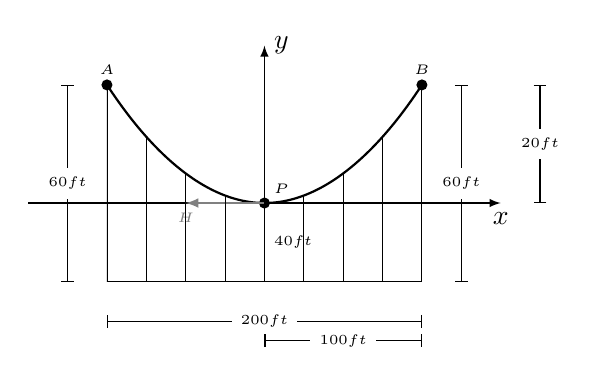
\begin{tikzpicture}[>=latex]
				\draw [->] (-3,1) -- (3,1) node [below] {\(x\)};
				\draw [->] (0,0) -- (0,3) node [right] {\(y\)};
				\draw [thick] (-2,2.5) node [above] {\tiny \(A\)} parabola bend (0,1) (2,2.5) node [above] {\tiny \(B\)};
				\fill (-2,2.5) circle (2pt) (2,2.5) circle (2pt);
				\fill (0,1) circle (2pt) node [above right] {\tiny \(P\)};
				\draw (-2,0) -- (2,0);
				\draw [|-|] (-2.5,0) to node [midway,fill=white] { \tiny\(60ft\)}++ (0,2.5);
				\draw [|-|] (2.5,0) to node [midway,fill=white] { \tiny\(60ft\)}++ (0,2.5);
				\draw [|-|] (-2,-0.5) to node [midway,fill=white] {\tiny \(200ft\)} ++ (4,0);
				\draw [|-|] (0,-0.75) to node [midway,fill=white] {\tiny \(100ft\)} ++ (2,0);
				\node [right] at (0,0.5) {\tiny \(40ft\)};
				\draw [|-|] (3.5,1) to node [midway,fill=white] {\tiny \(20ft\)} ++ (0,1.5);
				\draw [semithick,->, gray] (0,1) --++ (-1,0) node [below] {\tiny \(H\)};
				\clip (-2,0) -- (-2,2.5) parabola bend (0,1) (2,2.5) -- (2,0) -- cycle;
				\foreach \n in {-4,...,4} \draw (\n/2,0) --++ (0,3);
			\end{tikzpicture}
		\end{minipage}\hspace{5mm}
		\begin{minipage}{0.5\linewidth}
		\end{minipage}
\end{frame}
\begin{frame}[t]
\end{frame}

\begin{frame}[t]
	\begin{alertblock}{Ejercicio.}
		El puente de la figura del ejercicio anterior tiene ahora un peso variable de \(400+0.001x^2\), por pie de longitud, donde \(x\) es la distancia en pies desde el centro del puente. Encuentra una ecuación para la curva \(APB\).
	\end{alertblock}
\end{frame}
\begin{frame}[t]
\end{frame}

\begin{frame}[t]
	\begin{example}
		Considere una cuerd flexible de densidad constante \(\rho\) que cuelga de dos puntos fijos. Determina la forma de la cuerda.
	\end{example}
	\begin{minipage}{0.5\linewidth}
	\begin{tikzpicture}[>=latex]
		\draw [->] (-2,0) -- (2,0) node [below] {\(x\)};
		\draw [->] (0,-2) -- (0,2) node [right] {\(y\)};
		\coordinate (A) at (-1,1);
		\coordinate (B) at (1.4,1.4);
		\draw [thick , gray] (A) parabola bend (0,0) (B) node [below right] {\footnotesize con densidad \(\rho\)};
		\draw [dashed , gray] (1.3,0) --++ (0,1.2) --++ (-0.2,-0.3) --++ (0,-1) node [below] {\tiny \(\Delta x\)};
		\fill [red] (A) circle (1.5pt);
		\fill [red] (B) circle (1.5pt);
	\end{tikzpicture}
	\end{minipage}\hspace{5mm}
	\begin{minipage}{0.5\linewidth}
	\end{minipage}
\end{frame}

\begin{frame}[t]
	\begin{figure}[ht]
		\centering
		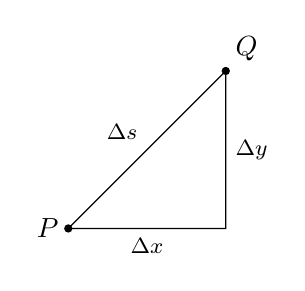
\begin{tikzpicture}[>=latex]
			\coordinate (P) at (0,0);
			\coordinate (Q) at (2,2);
			\coordinate (R) at (2,0);
			\fill (P) circle (1.5pt) node [left] {\(P\)};
			\fill (Q) circle (1.5pt) node [above right] {\(Q\)};
			\draw (P) to node [midway,above left] {\footnotesize\(\Delta s\)} 
			(Q) to node [midway,right] {\footnotesize\(\Delta y\)} 
			(R) to node [midway,below] {\footnotesize \(\Delta x\)} (P);
		\end{tikzpicture}
	\end{figure}
\end{frame}

\begin{frame}[t]
	\vspace{-5mm}
	\begin{example}
		Un cable pesa \(0.5\;lb/ft\) y cuelga de dos soportes que están a un mismo nivel a \(100ft\) de separación. Si la pendiente del cable n uno de los extremos es de \(12/5\).
		\begin{enumerate}
			\item Encuentre la tensión del cable en su punto más bajo.
			\item Determine la ecuación para la curva que forma el cable que cuelga.
			\item Encuentre la tensión en los soportes. 
		\end{enumerate}
	\end{example}
	\begin{figure}[ht]
		\centering
		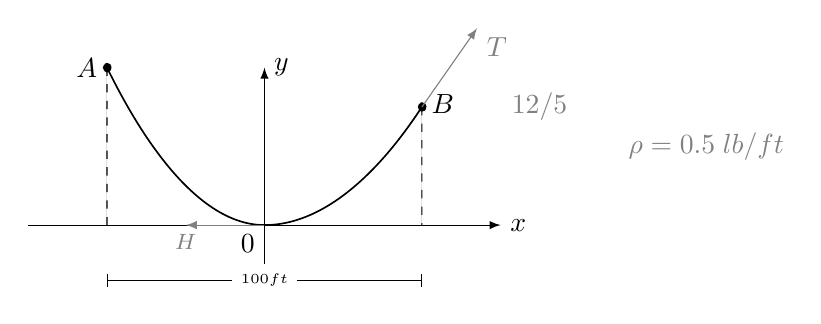
\begin{tikzpicture}[>=latex]
			\draw [->] (-3,0) -- (3,0) node [right] {\(x\)};
			\draw [->] (0,-0.5) -- (0,2) node [right] {\(y\)};
			\coordinate (A) at (-2,2);
			\coordinate (B) at (2,1.5);
			\draw [semithick] (A) parabola bend (0,0) (B);
			\filldraw [dashed] (A) circle (1.5pt) node [left] {\(A\)}--++ (0,-2);
			\filldraw [dashed] (B) circle (1.5pt) node [right] {\(B\) \hspace{5mm} \color{gray} \(12/5\)} --++ (0,-1.5);
			\node [below left] at (0,0) {\(0\)};
			\draw [gray,->] (0,0) -- (-1,0) node [below] {\footnotesize \(H\)};
			\draw [|-|] (-2,-0.7) to node [midway, fill=white] {\tiny \(100ft\)} ++ (4,0);
			\draw [->,gray] (B) --++ (0.7,1) node [below right] {\(T\)};
			\node [gray, right] at (4.5,1) {\(\rho =0.5\;lb/ft\)};
		\end{tikzpicture}
	\end{figure}
\end{frame}
\begin{frame}[t]
\end{frame}

\begin{frame}[t]
	\begin{enumerate}
		\item \hphantom{Usamos la condición}
	\begin{figure}[ht]
		\centering
		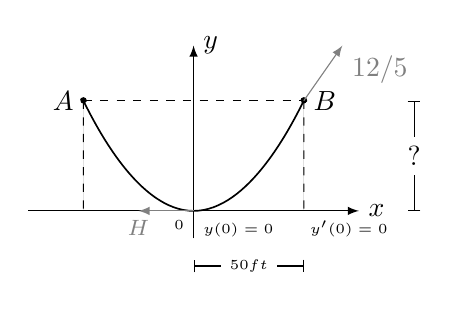
\begin{tikzpicture}[>=latex, scale=0.7]
			\draw [->] (-3,0) -- (3,0) node [right] {\(x\)};
			\draw [->] (0,-0.5) -- (0,3) node [right] {\(y\)};
			\coordinate (A) at (-2,2);
			\coordinate (B) at (2,2);
			\draw [semithick] (A) parabola bend (0,0) (B);
			\filldraw [dashed] (A) circle (1.5pt) node [left] {\(A\)}--++ (0,-2);
			\filldraw [dashed] (B) circle (1.5pt) node [right] {\(B\)} --++ (0,-2);
			\draw [dashed] (A) -- (B);
			\node [below left] at (0,0) {\tiny \(0\)};
			\node [below right] at (0,0) {\tiny \(y(0) =0\) \hspace{3mm} \(y'(0) =0\)};
			\draw [gray,->] (0,0) -- (-1,0) node [below] {\footnotesize \(H\)};
			\draw [|-|] (0,-1) to node [midway, fill=white] {\tiny \(50ft\)} ++ (2,0);
			\draw [->,gray] (B) --++ (0.7,1) node [below right] {\(12/5\)};
			\draw [|-|] (B) ++ (2,0) to node [midway,fill=white] {?} ++ (0,-2);
		\end{tikzpicture}
	\end{figure}
	\end{enumerate}
\end{frame}
% )))

\section{Deflexión de Vigas.} % (((
\begin{frame}[t]
	\frametitle{Deflexión de Vigas.}
	\begin{block}{}
		Considere una viga horizontal \(AB\), uniforme en su sección transversal y de material homogéneo.
		\begin{figure}[ht]
			\centering
			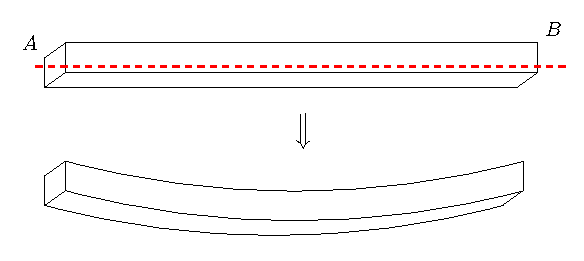
\includegraphics[width= 0.7 \linewidth]{IMAGENES_VIGAS/1/tikz.pdf}
		\end{figure}
		Hay diferentes maneras de apoyar las vigas.
	\end{block}
\end{frame}

\begin{frame}[t]
	\begin{block}{}
		Hay diferentes maneras de apoyar las vigas.
		\begin{figure}[ht]
			\centering
			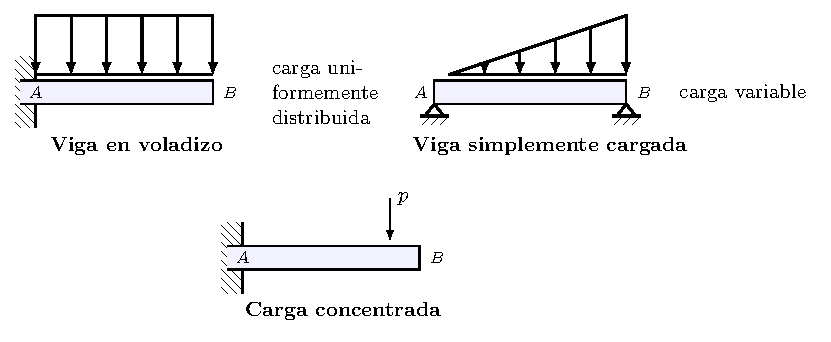
\includegraphics[width= \linewidth]{IMAGENES_VIGAS/2/tikz.pdf}
		\end{figure}
	\end{block}
\end{frame}

\begin{frame}[t]
	\begin{block}{Planteamiento de la E.D.}
		Considere una viga horizontal \(OB\) como se muestra a continuación.
		\begin{figure}[ht]
			\centering
			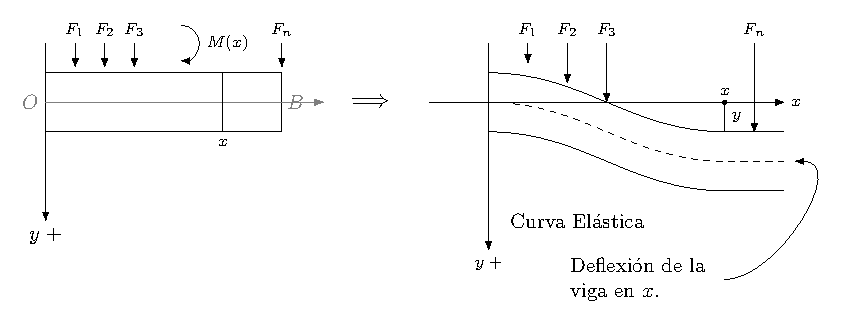
\includegraphics[width= \linewidth]{IMAGENES_VIGAS/3/tikz.pdf}
		\end{figure}
		Así pues, si determinamos la ecuación de la curva elástica, se conocerá la deflexión de la viga.
	\end{block}
\end{frame}

\begin{frame}[t]
	\begin{block}{}
		Definimos \(M(x)\) como el momento flexionante que corresponde a  la suma algebraica de los momentos de las fuerzas que actúan sobre un lado \(x\). Convención: Cuando las fuerzas se aplican hacia arriba producen un momento negativo, y cuando las fuerzas se aplican hacia abajo es positivo. \\[2mm]
		EL momento flexionante en \(x\) está relacionado con el radio de curvatura de la curva elástica en \(x\).\\
		\begin{minipage}{0.5\linewidth}
			\[
				M(x) = EI \dfrac{y''}{\big[1+(y') ^2\big] ^{3/2}}.
			\]
		\end{minipage}\hspace{5mm}
		\begin{minipage}{0.4\linewidth}
			\(E=\) módulo de elasticidad. \\
			\(I=\) momento de incercia.\\
			\(EI=\) rigidez flexural (constante).
		\end{minipage}
	\end{block}
\end{frame}

\begin{frame}[t]
	\vspace{-2mm}
	\begin{block}{}
		Suponiendo que la viga se dobla levemente, entonces la pendiente es tan pequeña que su cuadrado se puede despreciar comparado con \(1\). Luego
		\[
			M(x) = EI \;y''.
		\]
	\end{block}
	\vspace{-3mm}
	\begin{example}
		Una viga horizontal, simplemente apoyada de longitud \(L\), se dobla bajo su propio peso, el cuál es \(W\) por unidad de longitud. Encuentre la ecuación de su curva elástica.\\
		\begin{minipage}{0.6\linewidth}
			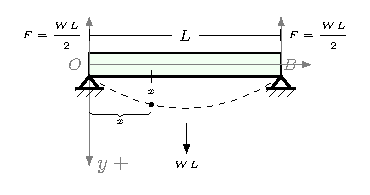
\includegraphics[width= \linewidth]{IMAGENES_VIGAS/4/tikz.pdf}
		\end{minipage}
		\begin{minipage}{0.3\linewidth}
			\footnotesize 
			Se tiene \(\dfrac{Peso}{U.\;long} =W\).\\[2mm]
			Balance de fuerzas.
			\[
				\begin{array}{rcl}
					\sum F_y & = & 0 \\[1mm]
					-F-F+WL & = & 0 \\[1mm]
					\iff -2F + WL & = & 0 \\[1mm]
					F & = & \dfrac{WL}{2}.
				\end{array}
			\]
		\end{minipage}
	\end{example}
\end{frame}

\begin{frame}[t]
	\begin{exampleblock}{}
		Determinemos el momento flexionante.
		\[
			\begin{array}{rcl}
				M(x) & = & -x \bigg(\dfrac{WL}{2}\bigg) + \bigg(\dfrac{x}{2}\bigg) (Wx) \\[5mm]
				M(x) & = & - \dfrac{W}{2} Lx + \dfrac{W}{2} x^2.
			\end{array}
		\]
		Luego, sustituyendo, \(M(x) =EI\;y''\),
		\[
			EI\;y'' = \dfrac{W}{2} Lx + \dfrac{W}{2} x^2.
		\]
		\(y(0) =0\), \(y(L) =0\).
		\[
			EI \; y'' = \dfrac{W}{2} x^2- \dfrac{WL}{2} x, \hspace{5mm} y(0) =0 \;,\; y(L) =0.
		\]
	\end{exampleblock}
\end{frame}

\begin{frame}[t]
	\vspace{-3mm}
	\begin{exampleblock}{}
		Integramos con respecto a \(x\). \vspace{-3mm}
		\newcommand{\dis}{\displaystyle} % este comando es sólo para no escribir la palabra \displaystyle completa :)
		\[
			\begin{array}{rcl}
				\dis\int EI\;y'' dx & = & \dis\int \bigg(\dfrac{W}{2} x^2- \dfrac{WL}{2} x\bigg) dx \\[5mm]
				\iff EI\;y' & = & \dfrac{W}{2} \dfrac{x^3}{3} - \dfrac{WL}{2} \dfrac{x^2}{2} +C, \\[5mm]
				\iff EI\;y' & = & \dfrac{W}{6} x^3- \dfrac{WL}{4} x^2+C, \vspace{-3mm}
			\end{array}
		\]
		Integramos nuevamente, \vspace{-3mm}
		\[
			\begin{array}{rcl}
				EI\;y & = & \dis\int EIy' dx = \dis\int \bigg(\dfrac{W}{6} - \dfrac{WL}{4} x^2+C_1\bigg) dx \\[5mm]
				\iff EI\;y & = & \dfrac{W}{24} x^4 - \dfrac{WL}{12} x^3C_1x+C_2 \vspace{-2mm}
			\end{array}
		\]
		\[
			\iff \color{red} \underline{\color{black}  y(x) = \dfrac{1}{EI} \bigg(\dfrac{W}{24} x^4- \dfrac{WL}{12} x^3+C_1x+C_2\bigg)}
		\]
	\end{exampleblock}
\end{frame}

\begin{frame}[t]
	\begin{exampleblock}{}
		Aplicamos la C.G. \(y(0) =0\), \(y(L) =0\).
		\footnotesize 
		\[
			\begin{array}{rcl}
				y(0) & = & \dfrac{1}{EI} \bigg(\dfrac{W}{24} (0) ^4- \dfrac{WL}{12} (0) ^3+C_1(0) +C_2\bigg) =0 \iff C_2 =0. \\[5mm]
				y(L) & = & \dfrac{1}{EI} \bigg(\dfrac{W}{24} L^4- \dfrac{WL}{12} L^3+C_1L+0\bigg) =0 \\[5mm] 
				\iff && \dfrac{W}{24} L^4 - \dfrac{WL^4}{12} +C_1L=0 \\[5mm]
				\iff && C_1 = \dfrac{WL^3}{24}.
			\end{array}
		\]
		Sustituyendo
		\begin{center}
			\color{red} \fbox{\(\color{black}  y(x) = \dfrac{1}{EI} \bigg(\dfrac{W}{24} x^4- \dfrac{WL}{12} x^3+ \dfrac{WL^3}{24}x\bigg)\)}
		\end{center} 
	\end{exampleblock}
\end{frame}

\begin{frame}[t]
	\begin{exampleblock}{}
		Encontremos la deflexión máxima de la viga, la cuál occurirá en \(L/2\).
		\[
			\begin{array}{rcl}
				y(L/2) & = & \dfrac{1}{EI} \bigg(\dfrac{WL}{24} \Big(\dfrac{L}{2}\Big) ^4- \dfrac{WL}{12} \Big(\dfrac{L}{2}\Big) ^3+ \dfrac{WL^3}{24} \Big(\dfrac{L}{2}\Big)\bigg) \\[6mm]
				\iff y_{max} & = & \dfrac{1}{EI} \bigg(\dfrac{5WL^4}{384}\bigg).
			\end{array}
		\]
	\end{exampleblock}

	\begin{example}
		Una viga uniforme horizontal simplemente apoyada de longitud \(L\) y peso despreciable, se dobla bajo la influencia de una carga concentrada \(\delta\), a una distancia de \(L/3\) de un extremo, como se muestra en la figura. Encuentre la ecuación de la curva elástica.
	\end{example}
\end{frame}

\begin{frame}[t]
	\begin{figure}[ht]
		\centering
		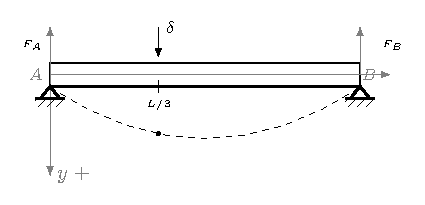
\includegraphics[width= \linewidth]{IMAGENES_VIGAS/5/tikz.pdf}
	\end{figure}
\end{frame}

\begin{frame}[t]
	\begin{alertblock}{Ejercicio.}
		Encontrar la curva elástica de una viga en voladizo uniforme de longitud \(L\), con un peso constante \(W\) por unidad de longitud. Determine la deflexión en el extremo libre.
	\end{alertblock}
	\begin{figure}[ht]
		\centering
		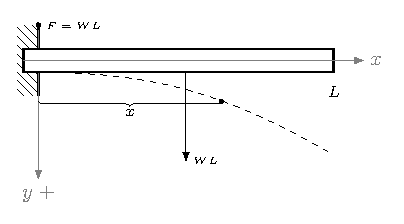
\includegraphics[width= \linewidth]{IMAGENES_VIGAS/6/tikz.pdf}
	\end{figure}
\end{frame}
% )))

\end{document}
